\documentclass[]{report}
\usepackage[T1]{fontenc}
\usepackage{lmodern}
\usepackage{amssymb,amsmath}
\usepackage{abstract}
\usepackage{ifxetex,ifluatex}
\usepackage{fixltx2e} % provides \textsubscript
%%foo
% use upquote if available, for straight quotes in verbatim environments
\IfFileExists{upquote.sty}{\usepackage{upquote}}{}
\ifnum 0\ifxetex 1\fi\ifluatex 1\fi=0 % if pdftex
  \usepackage[utf8]{inputenc}
\else % if luatex or xelatex
  \ifxetex
    \usepackage{mathspec}
    \usepackage{xltxtra,xunicode}
  \else
    \usepackage{fontspec}
  \fi
  \defaultfontfeatures{Mapping=tex-text,Scale=MatchLowercase}
  \newcommand{\euro}{€}
\fi
% use microtype if available
\IfFileExists{microtype.sty}{\usepackage{microtype}}{}
\usepackage{color}
\usepackage{fancyvrb}
\newcommand{\VerbBar}{|}
\newcommand{\VERB}{\Verb[commandchars=\\\{\}]}
\DefineVerbatimEnvironment{Highlighting}{Verbatim}{commandchars=\\\{\}}
% Add ',fontsize=\small' for more characters per line
\newenvironment{Shaded}{}{}
\newcommand{\KeywordTok}[1]{\textcolor[rgb]{0.00,0.44,0.13}{\textbf{{#1}}}}
\newcommand{\DataTypeTok}[1]{\textcolor[rgb]{0.56,0.13,0.00}{{#1}}}
\newcommand{\DecValTok}[1]{\textcolor[rgb]{0.25,0.63,0.44}{{#1}}}
\newcommand{\BaseNTok}[1]{\textcolor[rgb]{0.25,0.63,0.44}{{#1}}}
\newcommand{\FloatTok}[1]{\textcolor[rgb]{0.25,0.63,0.44}{{#1}}}
\newcommand{\ConstantTok}[1]{\textcolor[rgb]{0.53,0.00,0.00}{{#1}}}
\newcommand{\CharTok}[1]{\textcolor[rgb]{0.25,0.44,0.63}{{#1}}}
\newcommand{\SpecialCharTok}[1]{\textcolor[rgb]{0.25,0.44,0.63}{{#1}}}
\newcommand{\StringTok}[1]{\textcolor[rgb]{0.25,0.44,0.63}{{#1}}}
\newcommand{\VerbatimStringTok}[1]{\textcolor[rgb]{0.25,0.44,0.63}{{#1}}}
\newcommand{\SpecialStringTok}[1]{\textcolor[rgb]{0.73,0.40,0.53}{{#1}}}
\newcommand{\ImportTok}[1]{{#1}}
\newcommand{\CommentTok}[1]{\textcolor[rgb]{0.38,0.63,0.69}{\textit{{#1}}}}
\newcommand{\DocumentationTok}[1]{\textcolor[rgb]{0.73,0.13,0.13}{\textit{{#1}}}}
\newcommand{\AnnotationTok}[1]{\textcolor[rgb]{0.38,0.63,0.69}{\textbf{\textit{{#1}}}}}
\newcommand{\CommentVarTok}[1]{\textcolor[rgb]{0.38,0.63,0.69}{\textbf{\textit{{#1}}}}}
\newcommand{\OtherTok}[1]{\textcolor[rgb]{0.00,0.44,0.13}{{#1}}}
\newcommand{\FunctionTok}[1]{\textcolor[rgb]{0.02,0.16,0.49}{{#1}}}
\newcommand{\VariableTok}[1]{\textcolor[rgb]{0.10,0.09,0.49}{{#1}}}
\newcommand{\ControlFlowTok}[1]{\textcolor[rgb]{0.00,0.44,0.13}{\textbf{{#1}}}}
\newcommand{\OperatorTok}[1]{\textcolor[rgb]{0.40,0.40,0.40}{{#1}}}
\newcommand{\BuiltInTok}[1]{{#1}}
\newcommand{\ExtensionTok}[1]{{#1}}
\newcommand{\PreprocessorTok}[1]{\textcolor[rgb]{0.74,0.48,0.00}{{#1}}}
\newcommand{\AttributeTok}[1]{\textcolor[rgb]{0.49,0.56,0.16}{{#1}}}
\newcommand{\RegionMarkerTok}[1]{{#1}}
\newcommand{\InformationTok}[1]{\textcolor[rgb]{0.38,0.63,0.69}{\textbf{\textit{{#1}}}}}
\newcommand{\WarningTok}[1]{\textcolor[rgb]{0.38,0.63,0.69}{\textbf{\textit{{#1}}}}}
\newcommand{\AlertTok}[1]{\textcolor[rgb]{1.00,0.00,0.00}{\textbf{{#1}}}}
\newcommand{\ErrorTok}[1]{\textcolor[rgb]{1.00,0.00,0.00}{\textbf{{#1}}}}
\newcommand{\NormalTok}[1]{{#1}}
\usepackage{longtable,booktabs}
\usepackage{graphicx}
% Redefine \includegraphics so that, unless explicit options are
% given, the image width will not exceed the width of the page.
% Images get their normal width if they fit onto the page, but
% are scaled down if they would overflow the margins.
\makeatletter
\def\ScaleIfNeeded{%
  \ifdim\Gin@nat@width>\linewidth
    \linewidth
  \else
    \Gin@nat@width
  \fi
}
\makeatother
\let\Oldincludegraphics\includegraphics
{%
 \catcode`\@=11\relax%
 \gdef\includegraphics{\@ifnextchar[{\Oldincludegraphics}{\Oldincludegraphics[width=\ScaleIfNeeded]}}%
}%
\ifxetex
  \usepackage[setpagesize=false, % page size defined by xetex
              unicode=false, % unicode breaks when used with xetex
              xetex]{hyperref}
\else
  \usepackage[unicode=true]{hyperref}
\fi
\hypersetup{breaklinks=true,
            bookmarks=true,
            pdfauthor={Joshua Cook},
            pdftitle={Binary Classification via a Reinforcement Learner},
            colorlinks=true,
            citecolor=blue,
            urlcolor=blue,
            linkcolor=magenta,
            pdfborder={0 0 0}}
\urlstyle{same}  % don't use monospace font for urls
\setlength{\parindent}{0pt}
\setlength{\parskip}{6pt plus 2pt minus 1pt}
\setlength{\emergencystretch}{3em}  % prevent overfull lines
\setcounter{secnumdepth}{5}
\usepackage{fancyhdr}
\pagestyle{fancy}
\rhead{}

\title{Binary Classification via a Reinforcement Learner}
\author{Joshua Cook}
\date{}

\begin{document}
\maketitle

\begin{abstract}
{The purpose of this project is to solve a Kaggle competition using
manually constructed neural networks and reinforcement learning
techniques. The
\href{https://www.kaggle.com/c/predicting-red-hat-business-value}{competition}
in question is sponsored by Red Hat. Given situational (an ``action''
data set) and customer (a ``people'' data set) information, the goal is
to predict customer behavior for a given action. Customer behavior is a
binary classification; customers either take an action or they do not.
This project will use these two data sources and neural
network/reinforcement learning techniques to prepare an algorithm
capable of predicting outcomes against a third situational (a ``test
action'' data set) source. The infrastructure designed and built for
this project is informed by and informs the work,
\href{https://leanpub.com/thecontainerizedjupyterplatform}{\emph{the
Containerized Jupyter Platform}}. This work is accompanied by a set of
\href{http://joshuacook.me:8003/tree/ipynb}{Jupyter notebooks} and a
docker-compose.yml file that can be run in order to validate all
information here presented.}
\end{abstract}


{
\hypersetup{linkcolor=black}
\setcounter{tocdepth}{2}
\tableofcontents
}
\chapter{Definition}

Please refer to notebook
\href{http://joshuacook.me:8003/notebooks/ipynb/1\%20Definition.ipynb}{\texttt{1\ Definition}}.

\chapter{Problem Statement}\label{problem-statement}

In this Kaggle competition, Red Hat seeks an optimal algorithm for using
information about a given action and information about a given customer
to predict the customer's behavior with regard to that action. A
completed product will take the form of a csv with two items per row -
an \texttt{action\_id} from the test set, and a predicted outcome from
the set \({0,1}\).

The following is a sample of the required format for a solution
submission:

\begin{Shaded}
\begin{Highlighting}[]
\NormalTok{$ }\KeywordTok{head} \NormalTok{data/sample_submission.csv}

\KeywordTok{activity_id}\NormalTok{,outcome}
\KeywordTok{act1_1}\NormalTok{,0}
\KeywordTok{act1_100006}\NormalTok{,0}
\KeywordTok{act1_100050}\NormalTok{,0}
\KeywordTok{act1_100065}\NormalTok{,0}
\KeywordTok{act1_100068}\NormalTok{,0}
\KeywordTok{act1_100100}\NormalTok{,0}
\end{Highlighting}
\end{Shaded}

Data is provided in the form of three separate data sets encoded as CSV:

\begin{itemize}
\tightlist
\item
  \texttt{people.csv}
\item
  \texttt{act\_train.csv}
\item
  \texttt{act\_test.csv}.
\end{itemize}

We will store our data in two tables in a PostgreSQL Database. The
\texttt{action} (\texttt{act\_train.csv}) table makes reference to the
\texttt{people} (\texttt{people.csv}) table. Beyond this, the sets have
been scrubbed of any domain specific knowledge. Rather attributes are
referred to generically as \texttt{char\_1}, \texttt{char\_2}, etc. As
such the competition presents an interesting challenge, in which domain
knowledge is completely useless. The competition is in essence a ``pure
machine learning problem.''

\chapter{Approach}\label{approach}

We take the following approach to completing this task:

\begin{enumerate}
\def\labelenumi{\arabic{enumi}.}
\tightlist
\item
  Seed a PostgreSQL database with the three csv files.
\item
  One-Hot Encode the data and store the one-hot encoded vector as an
  array in the \texttt{action} table
\item
  Pull a batch of One-Hot Encoded vectors from the \texttt{action} table
  to pass to a Reinforcement Learner
\item
  Create, Update, and Store the parameters of the Reinforcement Learner
\item
  Use the Reinforcement Learner to run a set of predictions on Test
  Data.
\item
  Assess the accuracy of these predictions
\end{enumerate}

Note that while the Kaggle Challenge includes a set of test-data, for
the purposes of this study we will be holding a separate test set aside
that we are able to run our own local accuracy metrics. At the time of
this writing, the competion is closed to new submissions.

\chapter{Metrics}\label{metrics}

The quality of a solution to this task will be measured using the
following test error metric

\[\text{Ave}(I(y_i\neq\hat{y}_i))\]

Here, \(I\) is an indicator function which yields 0 if the predicted
outcome (\(\hat{y}_i\)) matches the actual outcome (\(y_i\)). While the
size of the dataset (over 2 million rows in the action set) makes this
problem atypical, it is at the end of the day, a binary classifcation
problem. As such this simple metric is sufficient to measure our
accuracy.

We will assess the learner against the test set throughout the training
process as a way of assessing the development of our learner. However,
the results of the development of the assessment will not be uses for
training and can thus be used repeatedly as an impartial measure of
progress.

\begin{figure}[htbp]
\centering
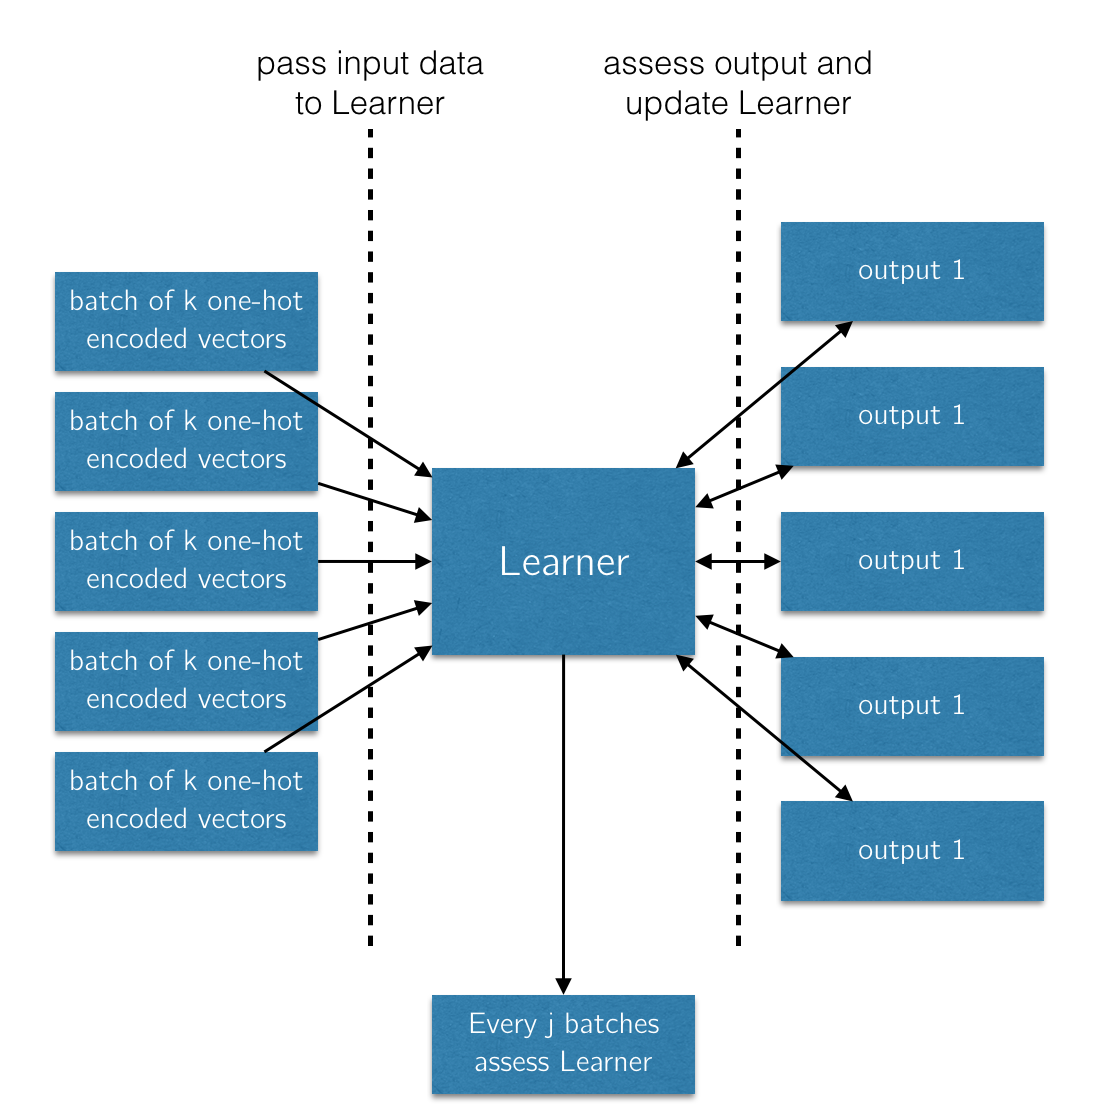
\includegraphics{assets/img/learner_diagram.png}
\caption{Learner Training and Assessment}
\end{figure}

\section{Infrastructure}\label{infrastructure}

We have designed a special infrastructure geared toward a
``back-end''/server-side implementation of our processes. This system
uses Jupyter notebooks as its main interface, thought it is possible to
interface with the system via the terminal. Additionally, a
browser-based control panel exists for tracking the progress of our
workers. We use to data management systems, a PostgreSQL database and
Redis. Finally, we have a worker layer of \(n\) scalable worker cpus
built using Python's \texttt{rq} framework.

\begin{figure}[htbp]
\centering
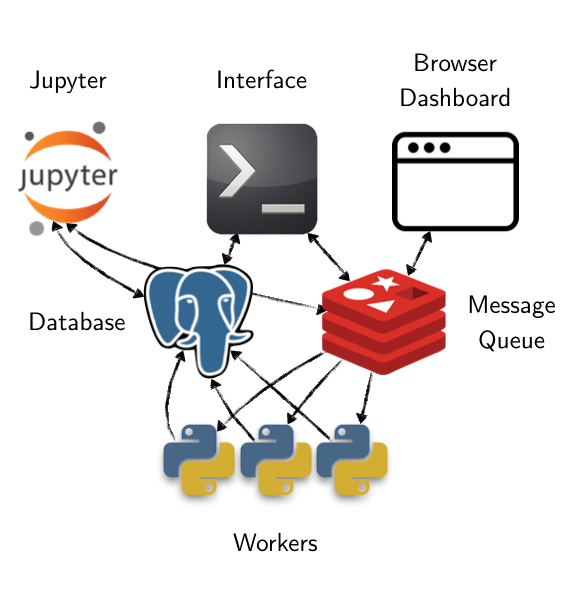
\includegraphics{assets/img/infrastructure.png}
\caption{Infrastructure}
\end{figure}

\chapter{Preliminary Data Analysis}

\chapter{Connecting to PostgreSQL}\label{connecting-to-postgresql}

Please refer to notebook
\href{http://joshuacook.me:8003/notebooks/ipynb/2.01\%20Preliminary\%20Data\%20Analysis\%20-\%20Connecting\%20to\%20PostgreSQL.ipynb}{\texttt{2.01\ Preliminary\ Data\ Analysis\ -\ Connecting\ to\ PostgreSQL}}.

We store all included data in a PostgreSQL database. By and large, we
access this database using the
\href{http://initd.org/psycopg/docs/}{\texttt{psycopg2}} library.

\begin{Shaded}
\begin{Highlighting}[]
\ImportTok{import} \NormalTok{psycopg2}

\ImportTok{from} \NormalTok{os }\ImportTok{import} \NormalTok{environ}
\NormalTok{conn }\OperatorTok{=} \NormalTok{psycopg2.}\ExtensionTok{connect}\NormalTok{(dbname}\OperatorTok{=}\StringTok{'postgres'}\NormalTok{, }
                        \NormalTok{user}\OperatorTok{=}\StringTok{'postgres'}\NormalTok{,}
                        \NormalTok{host}\OperatorTok{=}\NormalTok{environ[}\StringTok{'POSTGRES_1_PORT_5432_TCP_ADDR'}\NormalTok{])}
\NormalTok{cur }\OperatorTok{=} \NormalTok{conn.cursor()}
\end{Highlighting}
\end{Shaded}

\begin{Shaded}
\begin{Highlighting}[]
\NormalTok{cur.execute(}\StringTok{"SELECT COUNT(*) FROM people"}\NormalTok{)}\OperatorTok{;} \BuiltInTok{print}\NormalTok{(cur.fetchone())}
\NormalTok{cur.execute(}\StringTok{"SELECT COUNT(*) FROM action"}\NormalTok{)}\OperatorTok{;} \BuiltInTok{print}\NormalTok{(cur.fetchone())}
\end{Highlighting}
\end{Shaded}

\begin{verbatim}
(189118,)
(2695978,)
\end{verbatim}

\begin{Shaded}
\begin{Highlighting}[]
\NormalTok{conn.close()}
\end{Highlighting}
\end{Shaded}

\begin{figure}[htbp]
\centering
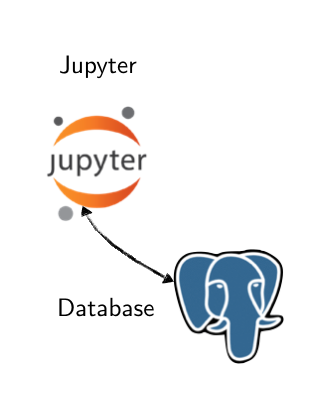
\includegraphics{assets/img/connecting_to_postgres.png}
\caption{Connecting to PostgreSQL}
\end{figure}

\pagebreak

\chapter{Data Exploration}\label{data-exploration}

The data to be used here consists of three datasets:

\begin{itemize}
\tightlist
\item
  \texttt{people.csv}
  \href{https://github.com/joshuacook/redhat/blob/master/data/people_head.csv}{sample}
\item
  \texttt{act\_train.csv}
  \href{https://github.com/joshuacook/redhat/blob/master/data/act_train_head.csv}{sample}
\item
  \texttt{act\_test.csv}
  \href{https://github.com/joshuacook/redhat/blob/master/data/act_test_head.csv}{sample}
\end{itemize}

We will do the following to analyze the datasets.

\begin{enumerate}
\def\labelenumi{\arabic{enumi}.}
\tightlist
\item
  seeding the database
\item
  basic postgres descriptor (\texttt{\textbackslash{}d+})
\item
  define the basic structure - rows, columns, data types
\item
  identify unique labels for each column and the counts for each label
\item
  run aggregates on columns - mean, median, max, min
\item
  identify duplicate records, if they exist
\item
  search for NULL data
\item
  create histograms of data
\end{enumerate}

\hypertarget{seeding-the-database}{\chapter{Seeding the
Database}\label{seeding-the-database}}

This is handled during the building of the Docker image for our
PostgreSQL database and is written into our database
\href{https://github.com/joshuacook/redhat/blob/master/docker/postgres/Dockerfile}{Dockerfile}.

In order to run the commands in this \texttt{Dockerfile} we use the
\texttt{docker-compose} tool to build our image.

\begin{Shaded}
\begin{Highlighting}[]
\NormalTok{$ }\KeywordTok{docker-compose} \NormalTok{build}
\end{Highlighting}
\end{Shaded}

During the building of the image, any \texttt{.sql} or \texttt{.sh}
files located in \texttt{/docker-entrypoint-initdb.d} will be executed.
We have defined the tables we will be using in the \texttt{tables.sql}
file. The structure will be shown in a moment when we run the postgres
descriptors. The full structure can be viewed in the seeding file
\href{https://github.com/joshuacook/redhat/blob/master/docker/postgres/tables.sql}{here}.
This functionality is part of the PostgreSQL public Docker image.

\pagebreak

\chapter{Basic PostgreSQL
Descriptors}\label{basic-postgresql-descriptors}

Having built and run our images, we now have a running PostgreSQL
database that has been seeded with our csv data.

\section{Descriptor for database}\label{descriptor-for-database}

We use the PostgreSQL descriptor command to display basic attributes of
our database.

\begin{verbatim}
postgres=# \d+
                          List of relations
 Schema |      Name       | Type  |  Owner   |  Size   | Description
--------+-----------------+-------+----------+---------+-------------
 public | action          | table | postgres | 235 MB  |
 public | people          | table | postgres | 30 MB   |
\end{verbatim}

\section{\texorpdfstring{Descriptor for \texttt{action}
table}{Descriptor for action table}}\label{descriptor-for-action-table}

We can repeat the same for a particular table. The tables have been
trimmed so as not to show columns of repeating type.

\begin{verbatim}
postgres=# \d+ action
           Table "public.action"
    Column    |            Type             | 
--------------+-----------------------------+
 people_id    | text                        | 
 act_id       | text                        | 
 act_date     | timestamp without time zone | 
 act_category | text                        | 
 act_char_1   | text                        | 
                   ...
 act_char_10  | text                        | 
 act_outcome  | boolean                     | 
Indexes:
    "action_pkey" PRIMARY KEY, btree (act_id)
Foreign-key constraints:
    "action_people_id_fkey" FOREIGN KEY (people_id) REFERENCES people(people_id)
\end{verbatim}

\pagebreak

\section{\texorpdfstring{Descriptor for \texttt{people}
table}{Descriptor for people table}}\label{descriptor-for-people-table}

\begin{verbatim}
postgres=# \d+ people
                Table "public.people"
   Column    |            Type             | Modifiers |
-------------+-----------------------------+-----------+
 people_id   | text                        | not null  |
 ppl_char_1  | text                        |           |
 ppl_group_1 | text                        |           |
 ppl_char_2  | text                        |           |
 ppl_date    | timestamp without time zone |           |
 ppl_char_3  | text                        |           |
                           ...
 ppl_char_9  | text                        |           |
 ppl_char_10 | boolean                     |           |
 ppl_char_11 | boolean                     |           |
 ppl_char_12 | boolean                     |           |
                           ...
 ppl_char_37 | boolean                     |           |
 ppl_char_38 | real                        |           |
Indexes:
    "people_pkey" PRIMARY KEY, btree (people_id)
Referenced by:
    TABLE "action" CONSTRAINT "action_people_id_fkey" 
        FOREIGN KEY (people_id) REFERENCES people(people_id)
\end{verbatim}

\pagebreak 

\chapter{Define the Basic Structure}\label{define-the-basic-structure}

Please refer to notebook
\href{http://joshuacook.me:8003/notebooks/ipynb/2.01\%20Preliminary\%20Data\%20Analysis\%20-\%20Define\%20the\%20Basic\%20Structure.ipynb}{\texttt{2.05\ Preliminary\ Data\ Analysis\ -\ Define\ the\ Basic\ Structure}}.

\textbf{TODO: Jupyter File}

The number of rows in a set can be identified by a query using the
\texttt{COUNT()} function. Our test and training sets can be identified
by the fact that the test set has \texttt{NULL} values in the
\texttt{act\_outcome} column.

\section{Number of Rows in database
tables}\label{number-of-rows-in-database-tables}

\begin{longtable}[]{@{}ccc@{}}
\toprule
database & number of rows & number of training rows\tabularnewline
\midrule
\endhead
\texttt{people} & 189118 & N/A\tabularnewline
\texttt{action} & 2695978 & 498687\tabularnewline
\bottomrule
\end{longtable}

\section{Number of Columns per Data
Type}\label{number-of-columns-per-data-type}

\begin{longtable}[]{@{}ccccl@{}}
\toprule
database & text & boolean & timestamp & real\tabularnewline
\midrule
\endhead
\texttt{people} & 11 & 28 & 1 & 0\tabularnewline
\texttt{action} & 13 & 1 & 1 & 1\tabularnewline
\bottomrule
\end{longtable}

\chapter{Identify Unique Labels}\label{identify-unique-labels}

\section{\texorpdfstring{Number of Unique Labels for
\texttt{people}}{Number of Unique Labels for people}}\label{number-of-unique-labels-for-people}

\begin{longtable}[]{@{}cl@{}}
\toprule
label & unique\tabularnewline
\midrule
\endhead
people\_id & 189118\tabularnewline
ppl\_group\_1 & 34224\tabularnewline
ppl\_date & 1196\tabularnewline
ppl\_char\_1 & 2\tabularnewline
ppl\_char\_2 & 3\tabularnewline
ppl\_char\_3 & 43\tabularnewline
ppl\_char\_4 & 25\tabularnewline
ppl\_char\_5 & 9\tabularnewline
ppl\_char\_6 & 7\tabularnewline
ppl\_char\_7 & 25\tabularnewline
ppl\_char\_8 & 8\tabularnewline
ppl\_char\_9 & 9\tabularnewline
\bottomrule
\end{longtable}

Additionally we do not show the final group of columns for the following
reasons. \texttt{ppl\_char\_10} through \texttt{ppl\_char\_37} are
boolean and have only two labels - \texttt{TRUE} and \texttt{FALSE}.

\texttt{ppl\_char\_38} is a continuous valued column.

\section{\texorpdfstring{Number of Unique Labels for
\texttt{action}}{Number of Unique Labels for action}}\label{number-of-unique-labels-for-action}

Again we first show columns that have too many labels. However, upon
second consideration we should use the column \texttt{act\_category}.

\begin{longtable}[]{@{}cc@{}}
\toprule
label & unique\tabularnewline
\midrule
\endhead
act\_id & 2695978\tabularnewline
act\_date & 411\tabularnewline
act\_category & 7\tabularnewline
act\_char\_1 & 51\tabularnewline
act\_char\_2 & 32\tabularnewline
act\_char\_3 & 11\tabularnewline
act\_char\_4 & 7\tabularnewline
act\_char\_5 & 7\tabularnewline
act\_char\_6 & 5\tabularnewline
act\_char\_7 & 8\tabularnewline
act\_char\_8 & 18\tabularnewline
act\_char\_9 & 19\tabularnewline
act\_char\_10 & 6969\tabularnewline
\bottomrule
\end{longtable}

We do not show the outcome \texttt{act\_outcome} because it is boolean.

\chapter{Run Aggregates on Columns}\label{run-aggregates-on-columns}

Next we take the average of our boolean columns. Note that all of them
skew to the negation, most of them heavily so. The only exception is
\texttt{act\_outcome} which, while still toward the negation, is closer
to the middle.

\begin{longtable}[]{@{}cc@{}}
\toprule
label & mean\tabularnewline
\midrule
\endhead
ppl\_char\_10 & (0.2509)\tabularnewline
ppl\_char\_11 & (0.2155)\tabularnewline
ppl\_char\_12 & (0.2403)\tabularnewline
ppl\_char\_13 & (0.3651)\tabularnewline
ppl\_char\_14 & (0.2598)\tabularnewline
ppl\_char\_15 & (0.2695)\tabularnewline
ppl\_char\_16 & (0.2821)\tabularnewline
ppl\_char\_17 & (0.2920)\tabularnewline
ppl\_char\_18 & (0.1876)\tabularnewline
ppl\_char\_19 & (0.2847)\tabularnewline
ppl\_char\_20 & (0.2291)\tabularnewline
ppl\_char\_21 & (0.2850)\tabularnewline
ppl\_char\_22 & (0.2911)\tabularnewline
ppl\_char\_23 & (0.2985)\tabularnewline
ppl\_char\_24 & (0.1904)\tabularnewline
ppl\_char\_25 & (0.3278)\tabularnewline
ppl\_char\_26 & (0.1670)\tabularnewline
ppl\_char\_27 & (0.2381)\tabularnewline
ppl\_char\_28 & (0.2889)\tabularnewline
ppl\_char\_29 & (0.1683)\tabularnewline
ppl\_char\_30 & (0.2069)\tabularnewline
ppl\_char\_31 & (0.2786)\tabularnewline
ppl\_char\_32 & (0.2849)\tabularnewline
ppl\_char\_33 & (0.2178)\tabularnewline
ppl\_char\_34 & (0.3565)\tabularnewline
ppl\_char\_35 & (0.2103)\tabularnewline
ppl\_char\_36 & (0.3437)\tabularnewline
ppl\_char\_37 & (0.2855)\tabularnewline
act\_outcome & (0.4440)\tabularnewline
\bottomrule
\end{longtable}

Then we take the average, maximum, and minimum of the single real-valued
column.

\begin{verbatim}
SELECT AVG(ppl_char_38), MAX(ppl_char_38), MIN(ppl_char_38) FROM people;
       avg        | max | min
------------------+-----+-----
 50.3273987669074 | 100 |   0
(1 row)
\end{verbatim}

\chapter{Identify Duplicate Records}\label{identify-duplicate-records}

Note that there are 189118 \texttt{people\_id} values, one for each row.
We can take this to mean that there are no duplicate entries in the
\texttt{people} dataset. The same is true with actions with 2695978
unique \texttt{act\_id} values.

\chapter{Search for NULL Data}\label{search-for-null-data}

There is null data in these datasets, in two locations. There are null
values in the boolean variables attached to the \texttt{action} table.
We will be handling this data, however, when we process the data for
handoff to the neural network. Additionally, there are null values in
the \texttt{act\_outcome} column, but this is functional as a null value
in this field signifies a \textbf{test} action as opposed to a
\textbf{train} action.

\pagebreak

\chapter{Create Histograms of Data}\label{create-histograms-of-data}

Please refer to notebook
\href{http://joshuacook.me:8003/notebooks/ipynb/2.10\%20Preliminary\%20Data\%20Analysis\%20-\%20Create\%20Histograms\%20of\%20Data.ipynb}{\texttt{2.10\ Preliminary\ Data\ Analysis\ -\ Create\ Histograms\ of\ Data}}.

Finally, we use the Python library
\href{https://stanford.edu/~mwaskom/software/seaborn/}{\texttt{seaborn}}
to create plots of our data as histograms.

First, we import the necessary libraries, then instantiate a connection
to our database.

\begin{Shaded}
\begin{Highlighting}[]
\ImportTok{import} \NormalTok{psycopg2}
\ImportTok{import} \NormalTok{numpy }\ImportTok{as} \NormalTok{np}
\ImportTok{import} \NormalTok{matplotlib.pyplot }\ImportTok{as} \NormalTok{plt}
\ImportTok{import} \NormalTok{seaborn }\ImportTok{as} \NormalTok{sns}
\OperatorTok{%}\NormalTok{matplotlib inline}

\ImportTok{from} \NormalTok{os }\ImportTok{import} \NormalTok{environ}
\NormalTok{conn }\OperatorTok{=} \NormalTok{psycopg2.}\ExtensionTok{connect}\NormalTok{(dbname}\OperatorTok{=}\StringTok{'postgres'}\NormalTok{, }
                        \NormalTok{user}\OperatorTok{=}\StringTok{'postgres'}\NormalTok{, }
                        \NormalTok{host}\OperatorTok{=}\NormalTok{environ[}\StringTok{'POSTGRES_1_PORT_5432_TCP_ADDR'}\NormalTok{])}
\NormalTok{cur }\OperatorTok{=} \NormalTok{conn.cursor()}
\end{Highlighting}
\end{Shaded}

\pagebreak

Next, we define a function that we will use to create numbered bins four
distinct labels for each column.

\begin{Shaded}
\begin{Highlighting}[]
\NormalTok{column }\OperatorTok{=} \StringTok{'ppl_char_1'}
\KeywordTok{def} \NormalTok{hist_buckets(column, table, cur):}
    \NormalTok{sql }\OperatorTok{=} \StringTok{"SELECT DISTINCT \{\} FROM \{\};"}\NormalTok{.}\BuiltInTok{format}\NormalTok{(column,table)}
    \NormalTok{cur.execute(sql)}

    \NormalTok{labels }\OperatorTok{=} \NormalTok{[}\BuiltInTok{str}\NormalTok{(l[}\DecValTok{0}\NormalTok{]) }\ControlFlowTok{for} \NormalTok{l }\OperatorTok{in} \NormalTok{cur.fetchall()]}
    \NormalTok{labels.sort()}
    \NormalTok{sql }\OperatorTok{=} \StringTok{"SELECT \{\} FROM "}\NormalTok{.}\BuiltInTok{format}\NormalTok{(}\StringTok{','}\NormalTok{.join(labels).replace(}\StringTok{' '}\NormalTok{,}\StringTok{'_'}\NormalTok{))}
    \NormalTok{sql_rows }\OperatorTok{=} \NormalTok{[}\StringTok{"""(SELECT COUNT(\{\}) }
\StringTok{                    FROM \{\} }
\StringTok{                    WHERE \{\} = '\{\}') as \{\}"""}\NormalTok{.}\BuiltInTok{format}\NormalTok{(column,}
                                                     \NormalTok{table,}
                                                     \NormalTok{column,}
                                                     \NormalTok{label,}
                                                     \NormalTok{label.replace(}\StringTok{' '}\NormalTok{,}\StringTok{'_'}\NormalTok{)) }
                                                     
                                                     \ControlFlowTok{for} \NormalTok{label }\OperatorTok{in} \NormalTok{labels]}

    \NormalTok{sql }\OperatorTok{+=} \StringTok{","}\NormalTok{.join(sql_rows)}
    
    \NormalTok{cur.execute(sql)}
    \NormalTok{bins }\OperatorTok{=} \NormalTok{cur.fetchall()[}\DecValTok{0}\NormalTok{]}
    \NormalTok{bins }\OperatorTok{=} \NormalTok{[}\BuiltInTok{int}\NormalTok{(bn.replace(}\StringTok{'('}\NormalTok{,}\StringTok{''}\NormalTok{).replace(}\StringTok{')'}\NormalTok{,}\StringTok{''}\NormalTok{)) }\ControlFlowTok{for} \NormalTok{bn }\OperatorTok{in} \NormalTok{bins]}
    \ControlFlowTok{return} \NormalTok{bins, labels}

\end{Highlighting}
\end{Shaded}

Then, we define a function to create our bar plot. We are using the
\texttt{seaborn} library which is designed to create beautiful plots
with minimal configuration.

\begin{Shaded}
\begin{Highlighting}[]
\KeywordTok{def} \NormalTok{bar_plot(col,table,cur):}
    \NormalTok{vals,labels }\OperatorTok{=} \NormalTok{hist_buckets(col,table,cur)}
    \NormalTok{x }\OperatorTok{=} \NormalTok{np.arange(}\BuiltInTok{len}\NormalTok{(vals))}
    \NormalTok{y }\OperatorTok{=} \NormalTok{np.array(vals)}
    \NormalTok{f }\OperatorTok{=} \NormalTok{plt.figure(figsize}\OperatorTok{=}\NormalTok{(}\DecValTok{12}\NormalTok{,}\DecValTok{3}\NormalTok{))}
    \NormalTok{ax }\OperatorTok{=} \NormalTok{f.add_axes([}\FloatTok{0.1}\NormalTok{, }\FloatTok{0.1}\NormalTok{, }\FloatTok{0.8}\NormalTok{, }\FloatTok{0.8}\NormalTok{])}
    \NormalTok{sns.barplot(x}\OperatorTok{=}\NormalTok{x, y}\OperatorTok{=}\NormalTok{y,palette}\OperatorTok{=}\StringTok{'Greens_d'}\NormalTok{)}
    \NormalTok{ax.set_title(}\StringTok{"Counts for \{\} in \{\}"}\NormalTok{.}\BuiltInTok{format}\NormalTok{(col,table))}
    \NormalTok{ax.set_xticks(x)}
    \NormalTok{ax.set_xticklabels([label.replace(}\StringTok{'type '}\NormalTok{,}\StringTok{''}\NormalTok{) }\ControlFlowTok{for} \NormalTok{label }\OperatorTok{in} \NormalTok{labels])}
\end{Highlighting}
\end{Shaded}

\begin{Shaded}
\begin{Highlighting}[]
\NormalTok{bar_plot(}\StringTok{'ppl_char_1'}\NormalTok{,}\StringTok{'people'}\NormalTok{,cur)}
\NormalTok{bar_plot(}\StringTok{'ppl_char_2'}\NormalTok{,}\StringTok{'people'}\NormalTok{,cur)}
\NormalTok{bar_plot(}\StringTok{'ppl_char_3'}\NormalTok{,}\StringTok{'people'}\NormalTok{,cur)}
\NormalTok{bar_plot(}\StringTok{'ppl_char_4'}\NormalTok{,}\StringTok{'people'}\NormalTok{,cur)}
\NormalTok{bar_plot(}\StringTok{'ppl_char_5'}\NormalTok{,}\StringTok{'people'}\NormalTok{,cur)}
\NormalTok{bar_plot(}\StringTok{'ppl_char_6'}\NormalTok{,}\StringTok{'people'}\NormalTok{,cur)}
\NormalTok{bar_plot(}\StringTok{'ppl_char_7'}\NormalTok{,}\StringTok{'people'}\NormalTok{,cur)}
\NormalTok{bar_plot(}\StringTok{'ppl_char_8'}\NormalTok{,}\StringTok{'people'}\NormalTok{,cur)}
\NormalTok{bar_plot(}\StringTok{'ppl_char_9'}\NormalTok{,}\StringTok{'people'}\NormalTok{,cur)}
\NormalTok{bar_plot(}\StringTok{'act_char_1'}\NormalTok{,}\StringTok{'action'}\NormalTok{,cur)}
\NormalTok{bar_plot(}\StringTok{'act_char_2'}\NormalTok{,}\StringTok{'action'}\NormalTok{,cur)}
\NormalTok{bar_plot(}\StringTok{'act_char_3'}\NormalTok{,}\StringTok{'action'}\NormalTok{,cur)}
\NormalTok{bar_plot(}\StringTok{'act_char_4'}\NormalTok{,}\StringTok{'action'}\NormalTok{,cur)}
\NormalTok{bar_plot(}\StringTok{'act_char_5'}\NormalTok{,}\StringTok{'action'}\NormalTok{,cur)}
\NormalTok{bar_plot(}\StringTok{'act_char_6'}\NormalTok{,}\StringTok{'action'}\NormalTok{,cur)}
\NormalTok{bar_plot(}\StringTok{'act_char_7'}\NormalTok{,}\StringTok{'action'}\NormalTok{,cur)}
\NormalTok{bar_plot(}\StringTok{'act_char_8'}\NormalTok{,}\StringTok{'action'}\NormalTok{,cur)}
\NormalTok{bar_plot(}\StringTok{'act_char_9'}\NormalTok{,}\StringTok{'action'}\NormalTok{,cur)}
\end{Highlighting}
\end{Shaded}

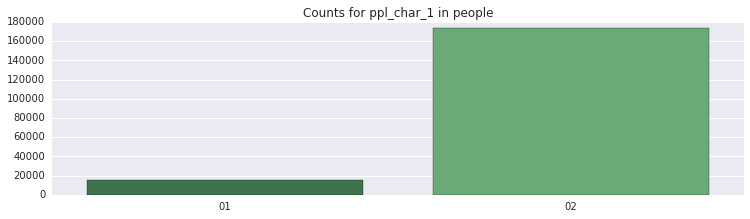
\includegraphics{assets/img/BarPlots_4_0.png}
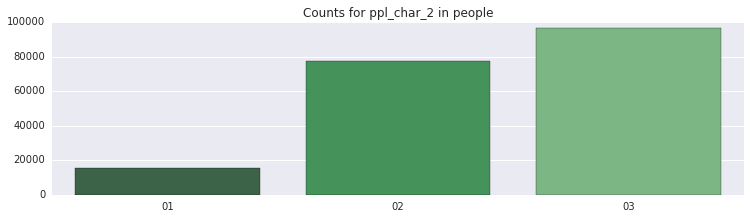
\includegraphics{assets/img/BarPlots_5_0.png}
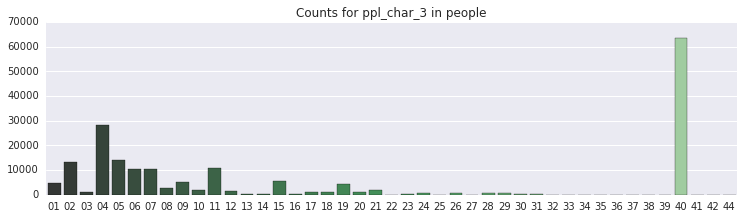
\includegraphics{assets/img/BarPlots_5_1.png}
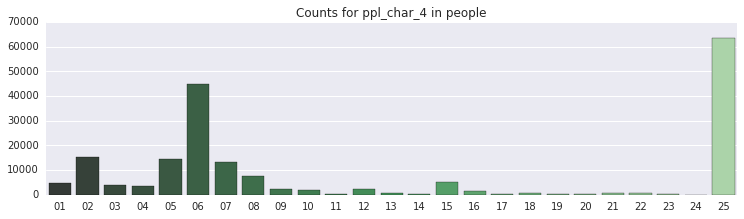
\includegraphics{assets/img/BarPlots_5_2.png}
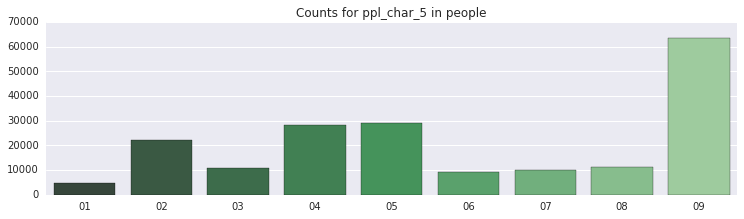
\includegraphics{assets/img/BarPlots_5_3.png}
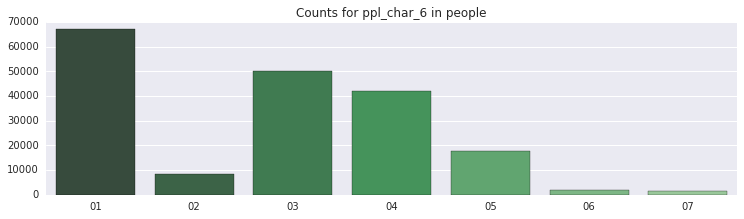
\includegraphics{assets/img/BarPlots_5_4.png}
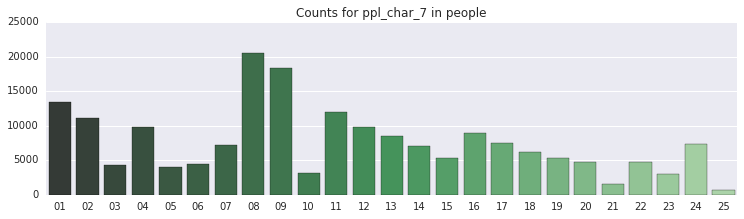
\includegraphics{assets/img/BarPlots_5_5.png}
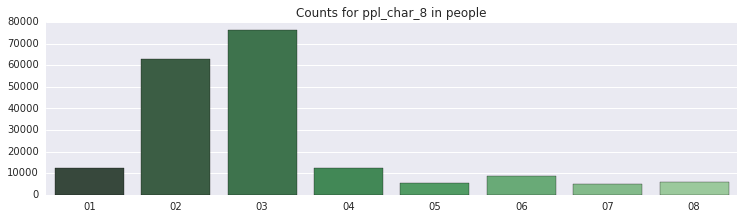
\includegraphics{assets/img/BarPlots_5_6.png}
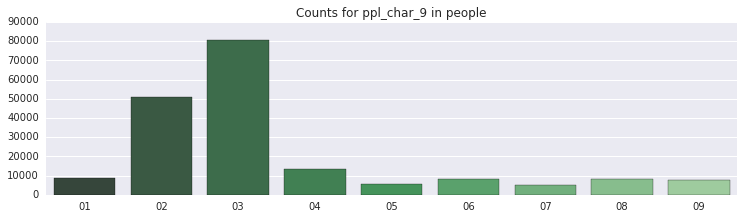
\includegraphics{assets/img/BarPlots_5_7.png}
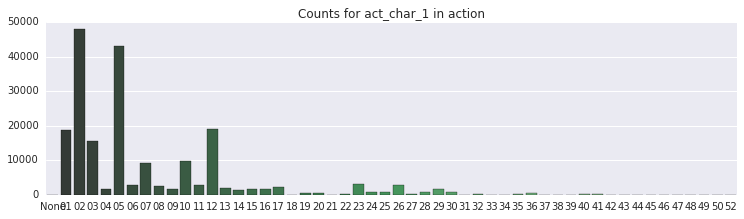
\includegraphics{assets/img/BarPlots_6_0.png}
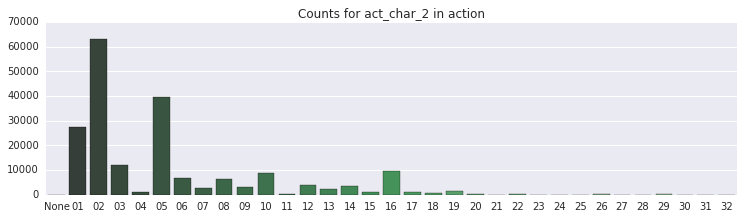
\includegraphics{assets/img/BarPlots_6_1.png}
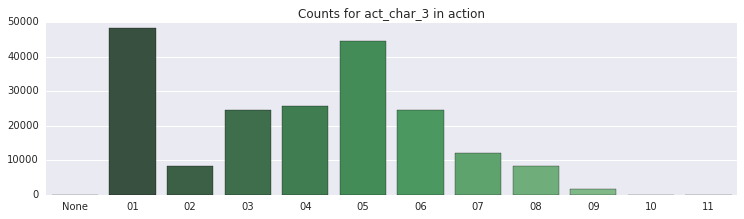
\includegraphics{assets/img/BarPlots_6_2.png}
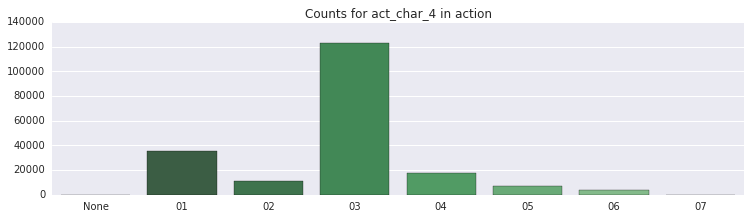
\includegraphics{assets/img/BarPlots_6_3.png}
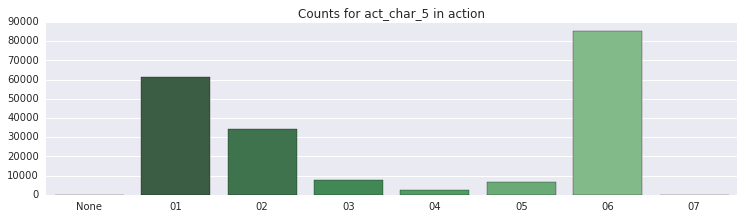
\includegraphics{assets/img/BarPlots_6_4.png}
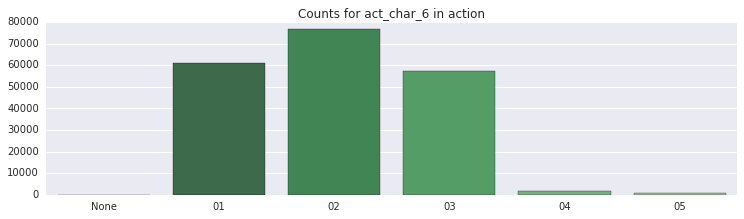
\includegraphics{assets/img/BarPlots_6_5.png}
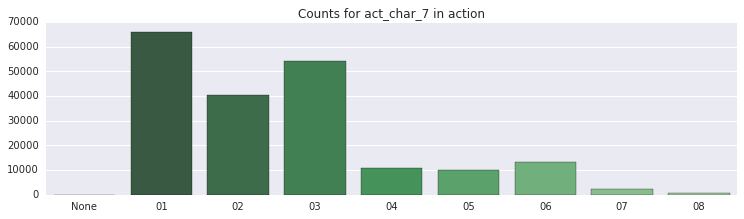
\includegraphics{assets/img/BarPlots_6_6.png}
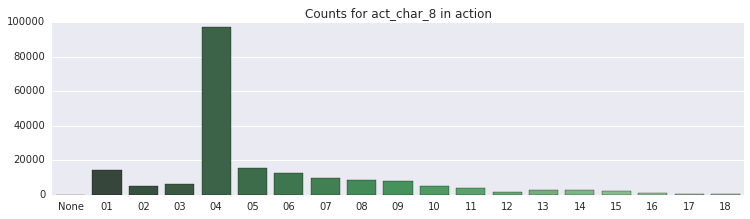
\includegraphics{assets/img/BarPlots_6_7.png}
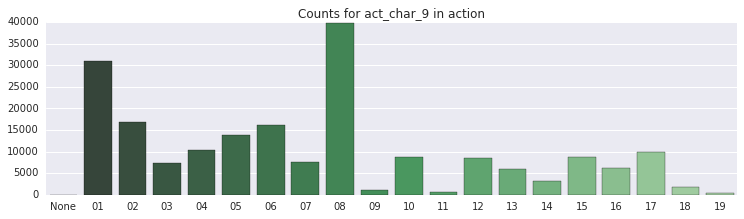
\includegraphics{assets/img/BarPlots_6_8.png}

\chapter{Algorithms and Techniques}

\chapter{One-Hot Encoding}\label{one-hot-encoding}

Please refer to notebook
\href{http://joshuacook.me:8003/notebooks/ipynb/3.01\%20Algorithms\%20and\%20Techniques\%20-\%20One-Hot\%20Encoding\%20Example.ipynb}{\texttt{3.01\ Algorithms\ and\ Techniques\ -\ One-Hot\ Encoding\ Example}}.

We will use the One-Hot Encoding algorithm to convert our categorical
data to numerical data. It may be tempting to merely convert our
categories to numbers i.e. \texttt{type\ 01} \(\to\) 1,
\texttt{type\ 02} \(\to\) 2, however, such an encoding of data implies a
linear relationship between our categories, where there may be none.

\begin{quote}
In one-hot encoding, a separate bit of state is used for each state. It
is called one-hot because only one bit is ``hot'' or TRUE at any time.
(Harris, David, and Sarah Harris. Digital design and computer
architecture. Elsevier, 2012.)
\end{quote}

This algorithm is also referred to as 1-of-K encoding. An example will
be helpful in illustrating the concept.

\pagebreak

\section{One-Hot Encoding Example}\label{one-hot-encoding-example}

\begin{Shaded}
\begin{Highlighting}[]
\ImportTok{import} \NormalTok{psycopg2}
\ImportTok{import} \NormalTok{numpy }\ImportTok{as} \NormalTok{np}
\ImportTok{from} \NormalTok{os }\ImportTok{import} \NormalTok{environ}
\NormalTok{conn }\OperatorTok{=} \NormalTok{psycopg2.}\ExtensionTok{connect}\NormalTok{(dbname}\OperatorTok{=}\StringTok{'postgres'}\NormalTok{, }
                        \NormalTok{user}\OperatorTok{=}\StringTok{'postgres'}\NormalTok{, }
                        \NormalTok{host}\OperatorTok{=}\NormalTok{environ[}\StringTok{'POSTGRES_1_PORT_5432_TCP_ADDR'}\NormalTok{])}
\NormalTok{cur }\OperatorTok{=} \NormalTok{conn.cursor()}

 \NormalTok{cur.execute(}\StringTok{"SELECT ppl_char_1,ppl_char_2 FROM people LIMIT 10"}\NormalTok{)}
\NormalTok{this_row }\OperatorTok{=} \NormalTok{cur.fetchone()}
\NormalTok{one_hot }\OperatorTok{=} \NormalTok{[]}
\ControlFlowTok{while} \NormalTok{this_row:}
    \NormalTok{one_hot.append([}
            \NormalTok{this_row[}\DecValTok{0}\NormalTok{] }\OperatorTok{==} \StringTok{'type 1'}\NormalTok{,}
            \NormalTok{this_row[}\DecValTok{0}\NormalTok{] }\OperatorTok{==} \StringTok{'type 2'}\NormalTok{,}
            \NormalTok{this_row[}\DecValTok{1}\NormalTok{] }\OperatorTok{==} \StringTok{'type 1'}\NormalTok{,}
            \NormalTok{this_row[}\DecValTok{1}\NormalTok{] }\OperatorTok{==} \StringTok{'type 2'}\NormalTok{,}
            \NormalTok{this_row[}\DecValTok{1}\NormalTok{] }\OperatorTok{==} \StringTok{'type 3'}\NormalTok{,}
        \NormalTok{])}
    \NormalTok{this_row }\OperatorTok{=} \NormalTok{cur.fetchone()}
\BuiltInTok{print}\NormalTok{(np.array(one_hot, dtype}\OperatorTok{=}\BuiltInTok{int}\NormalTok{))}

\NormalTok{[[}\DecValTok{0} \DecValTok{1} \DecValTok{0} \DecValTok{1} \DecValTok{0}\NormalTok{]}
 \NormalTok{[}\DecValTok{0} \DecValTok{1} \DecValTok{0} \DecValTok{0} \DecValTok{1}\NormalTok{]}
 \NormalTok{[}\DecValTok{0} \DecValTok{1} \DecValTok{0} \DecValTok{0} \DecValTok{1}\NormalTok{]}
 \NormalTok{[}\DecValTok{0} \DecValTok{1} \DecValTok{0} \DecValTok{0} \DecValTok{1}\NormalTok{]}
 \NormalTok{[}\DecValTok{0} \DecValTok{1} \DecValTok{0} \DecValTok{0} \DecValTok{1}\NormalTok{]}
 \NormalTok{[}\DecValTok{0} \DecValTok{1} \DecValTok{0} \DecValTok{0} \DecValTok{1}\NormalTok{]}
 \NormalTok{[}\DecValTok{0} \DecValTok{1} \DecValTok{0} \DecValTok{1} \DecValTok{0}\NormalTok{]}
 \NormalTok{[}\DecValTok{0} \DecValTok{1} \DecValTok{0} \DecValTok{0} \DecValTok{1}\NormalTok{]}
 \NormalTok{[}\DecValTok{0} \DecValTok{1} \DecValTok{0} \DecValTok{0} \DecValTok{1}\NormalTok{]}
 \NormalTok{[}\DecValTok{0} \DecValTok{1} \DecValTok{0} \DecValTok{0} \DecValTok{1}\NormalTok{]]}
 
\end{Highlighting}
\end{Shaded}

Here, we select two columns from our database. For each available type
for each column, we do a Boolean check and then cast this check to an
integer. The result is that for a given group of columns corresponding
to a single column in our original database, there will be a single
\texttt{1} and the remainder will be \texttt{0}. We use one-hot coding
because the categorical and boolean nature of the vast majority of our
data lends itself to this technique.

\chapter{Linear Classification via Neural
Network}\label{linear-classification-via-neural-network}

Linear classification will be the core algorithm upon which we will
build our neural network classifier. We borrow heavily for this approach
from Andrej Karpathy's
\href{http://cs231n.github.io/linear-classify/}{notes} for his
Convolutional Neural Networks course:

\begin{quote}
The approach will have two major components: a \textbf{score function}
that maps the raw data to class scores, and a \textbf{loss function}
that quantifies the agreement between the predicted scores and the
ground truth labels.
\end{quote}

\section{Score Function}\label{score-function}

We will develop a score function that maps input vectors to class scores

\[f: \mathbb{R^D} \mapsto \mathbb{R}^2\]

where \(D\) is the dimension of our one-hot encoded vectors and 2
represents the 2 classes of our binary classifier. Then,

\[f(x_i, W, b)=Wx_i+b=y\]

where \(x_i\) is a particular input vector, \(W\) is a matrix of weights
(dimension \(2 \times n\)), \(b\) is a bias vector, and \(y\) is a score
vector with a score for each class.

\begin{figure}[htbp]
\centering
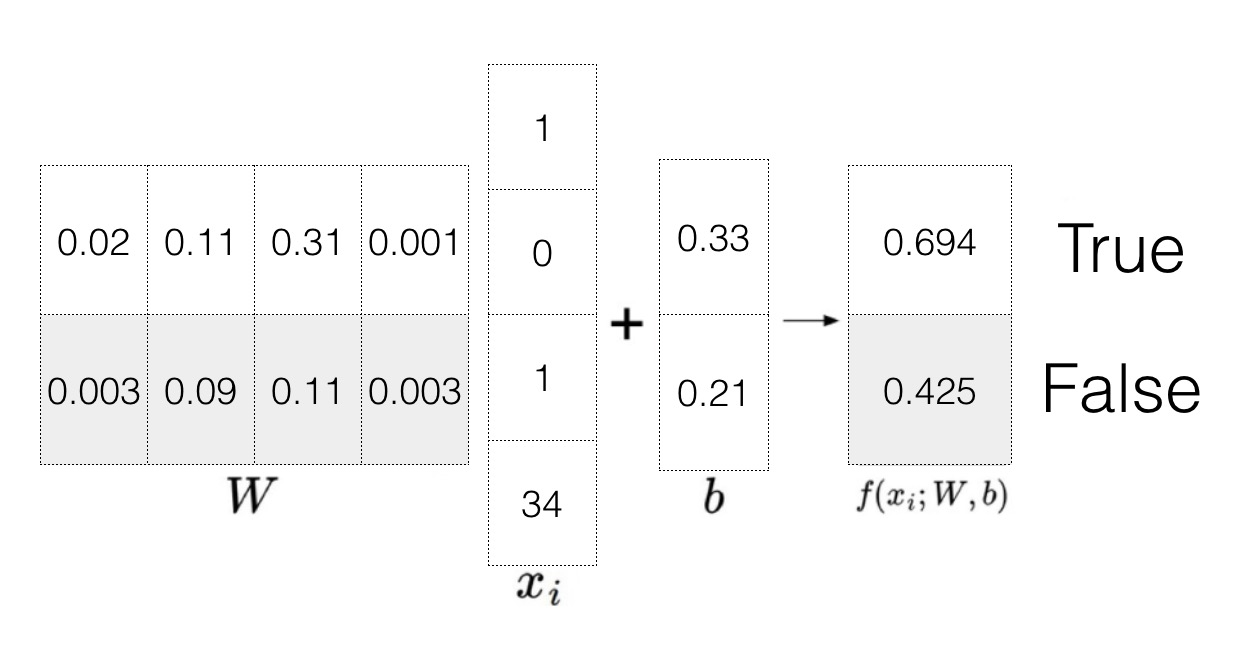
\includegraphics{assets/img/Linearclassifier.jpg}
\caption{}
\end{figure}

\section{Loss Function}\label{loss-function}

Note that of the inputs to our score function we do not have control
over the \(x_i\)s. Instead, we must change \(W\) and \(b\) to match a
set of given \(y\)s. To do this we will define a loss function that
measures our performance. We will use one of the most common loss
functions the multiclass support vector machine. Here the loss for a
given vector is

\[L_i=\sum_{j\neq y_i}\max(0,s_j-s_{y_i}+\Delta)\]

Here, \(s\) is the vector result of our score function and \(y_i\) is
the correct class. Our loss function computes a scalar value by
comparing each incorrect class score to the correct class score. We
expect the score of the correct class to be at least \(\Delta\) larger
than the score of each incorrect class.

\section{Regularization Penalty}\label{regularization-penalty}

It is possible that more than one set of weights could provide an
optimal response to our loss function. In order to prioritize the
smallest possible weights we will add a regularization penalty to our
loss function. Again we will go with a common technique and use the L2
norm.

\[R(W)=\sum_k\sum_lW^2_{k,l}\]

Additionally, including a regularizatiom penalty has the added benefit
of helping to prevent overfitting.

\section{Final Loss Function}\label{final-loss-function}

\[L=\frac{1}{N}\sum_iL_i+\lambda R(W)\]

Here, \(\lambda\) is a hyper parameter to be fit by cross-validation and
\(N\) is a batch size.

\chapter{Optimization}\label{optimization}

Possibile methods:

\section{Randomly guessing}\label{randomly-guessing}

\begin{itemize}
\tightlist
\item
  we initialize a weights matrix, \(W_{cur}\)
\item
  for each vector (or batch of vectors) passed to the learner, we
  generate a new weights matrix, \(W_{i}\)
\item
  if the new weights, \(W_{i}\) is better in score than \(W_{cur}\), we
  assign it to \(W_{cur}\) \[W_{cur} \to W_i\]
\item
  repeat for all of our test vectors
\end{itemize}

\section{Random Local Search}\label{random-local-search}

\begin{itemize}
\tightlist
\item
  we initilialize a weights matrix, \(W\)
\item
  for each batch of vectors passed, we generate a random matrix,
  \(\Delta W\), of the same dimension as \(W\) and scaled by some
  factor, \(\nu\)
\item
  we measure the loss against the sum \(W+\nu\Delta W\).
\item
  If \(W + \nu\Delta W\) has a better score than \(W\), we assign it to
  \(W\) \[W + \nu\Delta W \to W\]
\item
  repeat for all of our test vectors
\end{itemize}

\section{Gradient Descent}\label{gradient-descent}

\begin{itemize}
\tightlist
\item
  compute the best direction along which we should change our weight
  matrix that is mathematically guaranteed to be the direction of the
  steepest descent
\item
  the gradient is a vector of derivatives for each dimension in the
  input space
\item
  calculate the gradient and use this calculation to update the weight
  matrix \[W_{new} = W - \nabla L\]
\end{itemize}

\chapter{Benchmark}\label{benchmark}

The quality of a solution to this task will be measured using the
following test error metric

\[\text{Ave}(I(y_i\neq\hat{y}_i))\]

Here, \(I\) is an indicator function which yields 0 if the predicted
outcome (\(\hat{y}_i\)) matches the actual outcome (\(y_i\)), and
returns 1 otherwise. While the size of the dataset (over 2 million rows
in the action set) makes this problem atypical, it is at the end of the
day, a binary classification problem. As such this simple metric is
sufficient to measure our accuracy.

Of note is that, while the outcome is clearly defined by the contest,
for the purposes of this project, we will be using a portion of the
training set as our benchmark.

\chapter{Exploratory Visualization}

\chapter{Visualizing the Loss
Function}\label{visualizing-the-loss-function}

Please refer to notebook
\href{http://joshuacook.me:8003/notebooks/ipynb/4.01\%20Exploratory\%20Visualization\%20-\%20Visualizing\%20the\%20Loss\%20Function.ipynb}{\texttt{4.01\ Exploratory\ Visualization\ -\ Visualizing\ the\ Loss\ Function}}.

A relevant visualization to this task is that of the loss function. For
this visualizaton, we again turn to Andrej Karpathy's
\href{http://cs231n.github.io/optimization-1/}{notes}.

While we will have difficulty visualizing the loss function over the
complete weight space, we can visualize it over a smaller space to begin
to understand our approach.

\begin{Shaded}
\begin{Highlighting}[]
\ImportTok{import} \NormalTok{numpy }\ImportTok{as} \NormalTok{np}
\ImportTok{import} \NormalTok{matplotlib.pyplot }\ImportTok{as} \NormalTok{plt}
\ImportTok{import} \NormalTok{seaborn }\ImportTok{as} \NormalTok{sns}
\OperatorTok\NormalTok{matplotlib inline}
\end{Highlighting}
\end{Shaded}

For the purposes of this visualization, let us consider a small random
weight matrix \((2,p)\) for a binary classifier, i.e., one weight vector
for each classifier.

We then generate a random input vector \(x\) (with 6 parameters, and
then a trailing bias) and and a vector of outputs.

Finally, we randomly select a correct outcome for a binary classifier.

\begin{Shaded}
\begin{Highlighting}[]
\NormalTok{W }\OperatorTok{=} \NormalTok{np.random.rand(}\DecValTok{2}\NormalTok{,}\DecValTok{7}\NormalTok{)}
\NormalTok{x }\OperatorTok{=} \NormalTok{np.random.randint(}\DecValTok{2}\NormalTok{, size}\OperatorTok{=}\DecValTok{7}\NormalTok{)}
\NormalTok{x[}\DecValTok{6}\NormalTok{] }\OperatorTok{=} \DecValTok{1}
\NormalTok{correct_class }\OperatorTok{=} \NormalTok{np.random.randint(}\DecValTok{2}\NormalTok{)}
\end{Highlighting}
\end{Shaded}

\begin{Shaded}
\begin{Highlighting}[]
\NormalTok{W}
\end{Highlighting}
\end{Shaded}

\begin{verbatim}
array([[ 0.3,  0.5,  0.3,  0. ,  0.5,  0.1,  0.5],
       [ 0.8,  0.8,  0.1,  0.4,  0. ,  0.9,  0.5]])
\end{verbatim}

\begin{Shaded}
\begin{Highlighting}[]
\NormalTok{x}
\end{Highlighting}
\end{Shaded}

\begin{verbatim}
array([0, 0, 0, 0, 1, 1, 1])
\end{verbatim}

We then obtain our scores by multiplying

\[\texttt{scores}=Wx\]

The first score is for our first classifier, the second for the second
classifier. A score signifies how likely it is that the given classifier
is the correct classifier.

\begin{Shaded}
\begin{Highlighting}[]
\NormalTok{scores }\OperatorTok{=} \NormalTok{W.dot(x)}
\NormalTok{scores}
\end{Highlighting}
\end{Shaded}

\begin{verbatim}
array([ 1.2,  1.4])
\end{verbatim}

Next, we write a loss function for a single input vector.

\begin{Shaded}
\begin{Highlighting}[]
\ImportTok{from} \NormalTok{numpy.linalg }\ImportTok{import} \NormalTok{norm}
\KeywordTok{def} \NormalTok{loss_function_i(correct_class,x,W,delta}\OperatorTok{=}\FloatTok{1.0}\NormalTok{,gamma}\OperatorTok{=}\FloatTok{0.1}\NormalTok{):}
    \NormalTok{scores }\OperatorTok{=} \NormalTok{W.dot(x)}
    \NormalTok{correct_score }\OperatorTok{=} \NormalTok{scores[correct_class]}
    \NormalTok{margins }\OperatorTok{=} \NormalTok{np.maximum(}\DecValTok{0}\NormalTok{, scores }\OperatorTok{-} \NormalTok{correct_score }\OperatorTok{+} \NormalTok{delta)}
    \NormalTok{margins[correct_class] }\OperatorTok{=} \DecValTok{0}
    \ControlFlowTok{return} \NormalTok{np.}\BuiltInTok{sum}\NormalTok{(margins) }\OperatorTok{+} \NormalTok{gamma}\OperatorTok{*}\NormalTok{norm(W)}
\end{Highlighting}
\end{Shaded}

\begin{Shaded}
\begin{Highlighting}[]
\NormalTok{loss_function_i(correct_class,x,W)}
\end{Highlighting}
\end{Shaded}

\begin{verbatim}
0.9
\end{verbatim}

Finally, we vary the loss function for a single input with different
weights for a single parameter, \texttt{param}.

\begin{Shaded}
\begin{Highlighting}[]
\KeywordTok{def} \NormalTok{loss_function_in_a_direction(variable_weight,}
                                 \NormalTok{param,}
                                 \NormalTok{correct_class,}
                                 \NormalTok{x,W):}
    \NormalTok{delta_W }\OperatorTok{=} \NormalTok{np.zeros(W.shape)}
    \NormalTok{delta_W[:,param] }\OperatorTok{+=} \BuiltInTok{int}\NormalTok{(variable_weight)}\OperatorTok{*}\NormalTok{W[:,param]}
    \ControlFlowTok{return} \NormalTok{loss_function_i(correct_class,x,W}\OperatorTok{+}\NormalTok{delta_W)}
\end{Highlighting}
\end{Shaded}

\begin{Shaded}
\begin{Highlighting}[]
\NormalTok{loss_function_in_a_direction(}\DecValTok{1}\NormalTok{,}\DecValTok{1}\NormalTok{,correct_class,x,W)}
\end{Highlighting}
\end{Shaded}

\begin{verbatim}
1.0
\end{verbatim}

And then plot this function along various values of
\texttt{variable\_weight} for all of our \texttt{params} values.

\begin{Shaded}
\begin{Highlighting}[]
\KeywordTok{def} \NormalTok{plot_loss_function_for_a_single_parameter(plot_axis,param,correct_class,x,W):}
    \NormalTok{dependent_vector }\OperatorTok{=} \NormalTok{[loss_function_in_a_direction(variable_weight,}
                                                     \NormalTok{param,}
                                                     \NormalTok{correct_class,}
                                                     \NormalTok{x,W) }
                        \ControlFlowTok{for} \NormalTok{variable_weight }\OperatorTok{in} \BuiltInTok{range}\NormalTok{(}\OperatorTok{-}\DecValTok{20}\NormalTok{,}\DecValTok{20}\NormalTok{)]}
    \NormalTok{plot_axis.plot(}\BuiltInTok{range}\NormalTok{(}\OperatorTok{-}\DecValTok{20}\NormalTok{,}\DecValTok{20}\NormalTok{),dependent_vector)}
    
\KeywordTok{def} \NormalTok{render_all_plots(correct_class,x,W):}
    \NormalTok{figure, axes }\OperatorTok{=} \NormalTok{plt.subplots(}\DecValTok{1}\NormalTok{,}\DecValTok{7}\NormalTok{, sharex}\OperatorTok{=}\VariableTok{True}\NormalTok{, sharey}\OperatorTok{=}\VariableTok{True}\NormalTok{, figsize}\OperatorTok{=}\NormalTok{(}\DecValTok{20}\NormalTok{,}\DecValTok{6}\NormalTok{))}
    \ControlFlowTok{for} \NormalTok{param, axis }\OperatorTok{in} \BuiltInTok{zip}\NormalTok{(}\BuiltInTok{range}\NormalTok{(}\DecValTok{7}\NormalTok{),axes):}
        \NormalTok{plot_loss_function_for_a_single_parameter(axis,param,correct_class,x,W)    }
\end{Highlighting}
\end{Shaded}

\begin{Shaded}
\begin{Highlighting}[]
\NormalTok{render_all_plots(correct_class,x,W)}
\end{Highlighting}
\end{Shaded}

\begin{figure}[htbp]
\centering
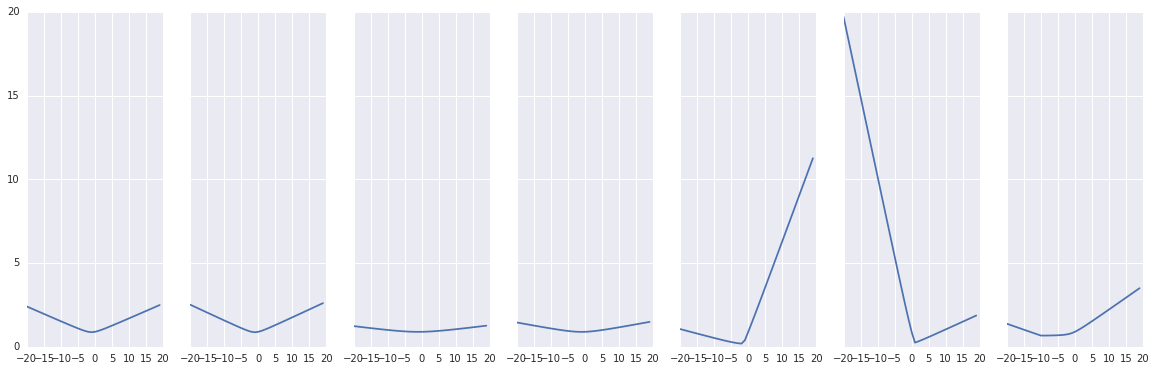
\includegraphics{assets/img/loss_function_one_param.png}
\caption{Visualizing Loss Function change along one Parameter}
\end{figure}

It is of note that every parameter is convex and can be minimized.

\begin{Shaded}
\begin{Highlighting}[]
\KeywordTok{def} \NormalTok{loss_function_in_two_directions(a,p_1,b,p_2,correct_class,x,W):}
    \NormalTok{delta_W }\OperatorTok{=} \NormalTok{np.zeros(W.shape)}
    \NormalTok{delta_W[:,p_1] }\OperatorTok{+=} \BuiltInTok{int}\NormalTok{(a)}\OperatorTok{*}\NormalTok{W[:,p_1]}
    \NormalTok{delta_W[:,p_2] }\OperatorTok{+=} \BuiltInTok{int}\NormalTok{(b)}\OperatorTok{*}\NormalTok{W[:,p_2]}
    \ControlFlowTok{return} \NormalTok{loss_function_i(correct_class,x,W}\OperatorTok{+}\NormalTok{delta_W)}

\end{Highlighting}
\end{Shaded}

We can also do the same for a comparison of two varied parameters.
Again, note that each of these plots is convex.

\begin{Shaded}
\begin{Highlighting}[]
\KeywordTok{def} \NormalTok{build_heat_map_for_two_parameters(p_1,p_2,min_val,max_val,nx,correct,x,W):}
    \NormalTok{X }\OperatorTok{=} \NormalTok{np.linspace(min_val, max_val, nx)}
    \NormalTok{Y }\OperatorTok{=} \NormalTok{np.linspace(min_val, max_val, nx)}
    \ControlFlowTok{return} \NormalTok{[[loss_function_in_two_directions(xv,p_1,yv,p_2,correct,x,W)}
             \ControlFlowTok{for} \NormalTok{xv }\OperatorTok{in} \NormalTok{X]}
            \ControlFlowTok{for} \NormalTok{yv }\OperatorTok{in} \NormalTok{Y]}
\end{Highlighting}
\end{Shaded}

\begin{Shaded}
\begin{Highlighting}[]
\KeywordTok{def} \NormalTok{plot_heatmap(plot_axis,p_1,p_2,correct,x,W):}
    \NormalTok{this_heat_map }\OperatorTok{=} \NormalTok{build_heat_map_for_two_parameters(p_1,p_2,}\OperatorTok{-}\DecValTok{100}\NormalTok{,}\DecValTok{100}\NormalTok{,}\DecValTok{50}\NormalTok{,correct,x,W)}
    \NormalTok{sns.heatmap(this_heat_map,}
                \NormalTok{cmap}\OperatorTok{=}\StringTok{'autumn'}\NormalTok{, }
                \NormalTok{cbar}\OperatorTok{=}\VariableTok{False}\NormalTok{, }
                \NormalTok{xticklabels}\OperatorTok{=}\VariableTok{False}\NormalTok{, }
                \NormalTok{yticklabels}\OperatorTok{=}\VariableTok{False}\NormalTok{, }
                \NormalTok{vmin}\OperatorTok{=}\DecValTok{0}\NormalTok{,vmax}\OperatorTok{=}\DecValTok{5}\NormalTok{,}
                \NormalTok{ax}\OperatorTok{=}\NormalTok{plot_axis)}
    
\KeywordTok{def} \NormalTok{render_all_plots(correct_class,x,W):}
    \NormalTok{plt.figure(figsize}\OperatorTok{=}\NormalTok{(}\DecValTok{18}\NormalTok{,}\DecValTok{21}\NormalTok{))}
    \NormalTok{figure, axes }\OperatorTok{=} \NormalTok{plt.subplots(}\DecValTok{7}\NormalTok{,}\DecValTok{6}\NormalTok{, sharex}\OperatorTok{=}\VariableTok{True}\NormalTok{, sharey}\OperatorTok{=}\VariableTok{True}\NormalTok{, figsize}\OperatorTok{=}\NormalTok{(}\DecValTok{18}\NormalTok{,}\DecValTok{21}\NormalTok{))}
    \ControlFlowTok{for} \NormalTok{p_1, axes_i }\OperatorTok{in} \BuiltInTok{zip}\NormalTok{(}\BuiltInTok{range}\NormalTok{(}\DecValTok{7}\NormalTok{),axes):        }
        \NormalTok{p_2s }\OperatorTok{=} \NormalTok{[i }\ControlFlowTok{for} \NormalTok{i }\OperatorTok{in} \BuiltInTok{range}\NormalTok{(}\DecValTok{7}\NormalTok{)]}
        \NormalTok{p_2s.remove(p_1) }
        \ControlFlowTok{for} \NormalTok{p_2, axis }\OperatorTok{in} \BuiltInTok{zip}\NormalTok{(p_2s, axes_i):}
            \NormalTok{plot_heatmap(axis,p_1,p_2,correct_class,x,W)}
            \NormalTok{axis.set_title(}\StringTok{"p \{\} v p \{\}"}\NormalTok{.}\BuiltInTok{format}\NormalTok{(}\BuiltInTok{str}\NormalTok{(p_1),}\BuiltInTok{str}\NormalTok{(p_2)))}
\end{Highlighting}
\end{Shaded}

\begin{Shaded}
\begin{Highlighting}[]
\NormalTok{render_all_plots(correct_class,x,W)}
\end{Highlighting}
\end{Shaded}

\begin{verbatim}
<matplotlib.figure.Figure at 0x7f676d94f9b0>
\end{verbatim}

\begin{figure}[htbp]
\centering
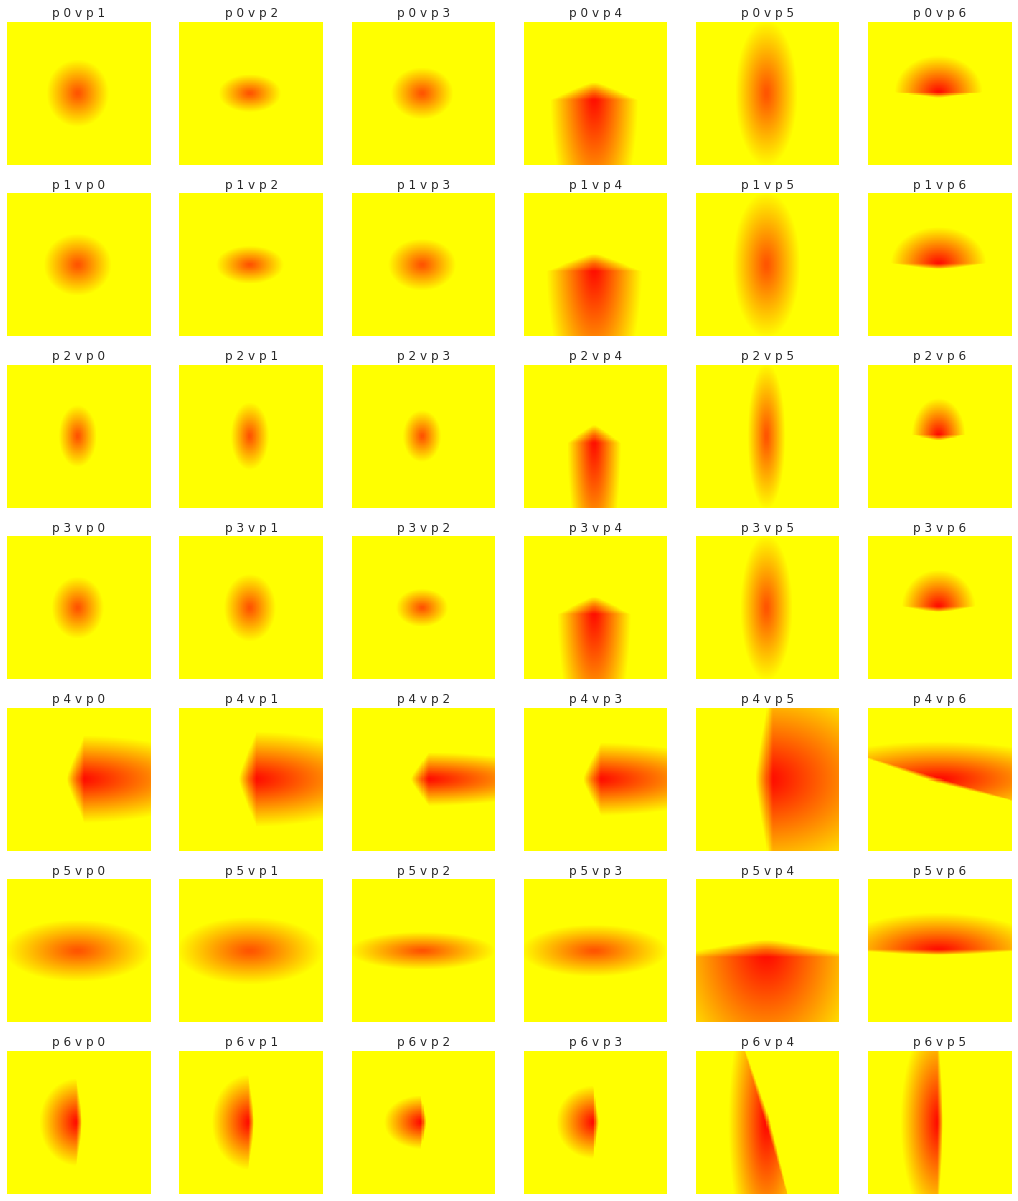
\includegraphics{assets/img/loss_function_two_params.png}
\caption{Visualizing Loss Function change against Two Parameters}
\end{figure}

\chapter{Data Preprocessing}

\chapter{CSV Manipulation}\label{csv-manipulation}

The dataset was a set provided by Kaggle. As such, it was already well
structured and clean. Still, in order to facilitate processing, some
work had to be done on the csv data itself.

\section{\texorpdfstring{\texttt{act\_train.csv}}{act\_train.csv}}\label{act_train.csv}

An additional column had to be added to the csv in order to ultimately
provide a null space in which to insert our
\texttt{act\_one\_hot\_encoded} binary value. This was done via the
\texttt{sed} command line tool by adding a comma to each line.

\begin{Shaded}
\begin{Highlighting}[]
\NormalTok{$ }\KeywordTok{sed} \NormalTok{-e }\StringTok{'s/$/,/'} \NormalTok{-i act_train.csv }\KeywordTok{>} \NormalTok{new_act_train.csv }
\end{Highlighting}
\end{Shaded}

\section{\texorpdfstring{\texttt{act\_test.csv}}{act\_test.csv}}\label{act_test.csv}

For the test data set, we needed to add two columns, one for the null
outcome (test and train are stored in the same table and distinguished
by having a true, false or null value) and the same null space in which
to insert the \texttt{act\_one\_hot\_encoded} binary value.

\begin{Shaded}
\begin{Highlighting}[]
\NormalTok{$ }\KeywordTok{sed} \NormalTok{-e }\StringTok{'s/$/,/'} \NormalTok{-i act_test.csv }\KeywordTok{>} \NormalTok{new_act_test.csv }
\end{Highlighting}
\end{Shaded}

\section{All Sets}\label{all-sets}

Additionally, we wanted to convert all attributes to double digit
attributes i.e. \texttt{char\ 1} \(\to\) \texttt{char\ 01}.

\begin{Shaded}
\begin{Highlighting}[]
\NormalTok{$ }\KeywordTok{sed} \NormalTok{-e }\StringTok{'s/,char (\textbackslash{}d),/,char 0\textbackslash{}1,/'} \NormalTok{-i act_train.csv }\KeywordTok{>} \NormalTok{new_act_train.csv}
\end{Highlighting}
\end{Shaded}

\textbf{In this section, all of your preprocessing steps will need to be
clearly documented, if any were necessary. From the previous section,
any of the abnormalities or characteristics that you identified about
the dataset will be addressed and corrected here. Questions to ask
yourself when writing this section:}

\chapter{One-Hot Encoding}\label{one-hot-encoding-1}

We will be storing our one-hot encoded numpy arrays as binary data in
the \texttt{action} table column \texttt{act\_one\_hot\_encoded}. Here
is a minimal implementation of this.

\begin{Shaded}
\begin{Highlighting}[]
\ImportTok{import} \NormalTok{psycopg2}
\ImportTok{import} \NormalTok{numpy }\ImportTok{as} \NormalTok{np}
\ImportTok{from} \NormalTok{os }\ImportTok{import} \NormalTok{environ}
\NormalTok{conn }\OperatorTok{=} \NormalTok{psycopg2.}\ExtensionTok{connect}\NormalTok{(dbname}\OperatorTok{=}\StringTok{'postgres'}\NormalTok{, }
                        \NormalTok{user}\OperatorTok{=}\StringTok{'postgres'}\NormalTok{,}
                        \NormalTok{host}\OperatorTok{=}\NormalTok{environ[}\StringTok{'POSTGRES_1_PORT_5432_TCP_ADDR'}\NormalTok{])}
\NormalTok{cur }\OperatorTok{=} \NormalTok{conn.cursor()}

\KeywordTok{def} \NormalTok{update_one_hot_encoding(vector, action_id):}
    \NormalTok{sql }\OperatorTok{=} \StringTok{"""}
\StringTok{        UPDATE action }
\StringTok{        SET act_one_hot_encoding = \{\}}
\StringTok{        WHERE act_id='\{\}'}
\StringTok{        """}\NormalTok{.}\BuiltInTok{format}\NormalTok{(psycopg2.Binary(vector), action_id)}
    \NormalTok{cur.execute(sql)}
    \NormalTok{conn.commit()}
    
\NormalTok{eye_3 }\OperatorTok{=} \NormalTok{np.eye(}\DecValTok{3}\NormalTok{)}

\NormalTok{update_one_hot_encoding(conn, cur, eye_4, action_id)}
\end{Highlighting}
\end{Shaded}

Next, we verify that the vector was properly stored.

\begin{Shaded}
\begin{Highlighting}[]
\KeywordTok{def} \NormalTok{fetch_one_hot_encoding(conn, cur, action_id):}
    \NormalTok{sql }\OperatorTok{=} \StringTok{"""}
\StringTok{        SELECT act_one_hot_encoding}
\StringTok{        FROM action}
\StringTok{        WHERE act_id='\{\}'}
\StringTok{        """}\NormalTok{.}\BuiltInTok{format}\NormalTok{(action_id)}
    \NormalTok{cur.execute(sql)}
    \NormalTok{buf }\OperatorTok{=} \NormalTok{cur.fetchone()[}\DecValTok{0}\NormalTok{]}
    \ControlFlowTok{return} \NormalTok{np.frombuffer(buf)}
    


\NormalTok{fetch_one_hot_encoding(conn, cur, action_id)}
\NormalTok{array([ }\DecValTok{1}\NormalTok{.,  }\DecValTok{0}\NormalTok{.,  }\DecValTok{0}\NormalTok{.,  }\DecValTok{0}\NormalTok{.,  }\DecValTok{1}\NormalTok{.,  }\DecValTok{0}\NormalTok{.,  }\DecValTok{0}\NormalTok{.,  }\DecValTok{0}\NormalTok{.,  }\DecValTok{1}\NormalTok{.])}
\end{Highlighting}
\end{Shaded}

\chapter{Implementation}

\chapter{Steps to Implementation}\label{steps-to-implementation}

\begin{enumerate}
\def\labelenumi{\arabic{enumi}.}
\tightlist
\item
  Seed a PostgreSQL database with the three csv files.
\item
  One-Hot Encode the data and store the one-hot encoded vector as an
  array in the \texttt{action} table
\item
  Train and Assess a Series of Learners
\item
  Random Weight Matrix with No Training
\item
  Random Search
\end{enumerate}

\chapter{Seed a PostgreSQL database with the three csv
files.}\label{seed-a-postgresql-database-with-the-three-csv-files.}

This step is done at instantiation of the system. Refer to
\protect\hyperlink{seeding-the-database}{Seeding the Database}.

\chapter{\texorpdfstring{One-Hot Encode the data and store the one-hot
encoded vector as an array in the \texttt{action}
table}{One-Hot Encode the data and store the one-hot encoded vector as an array in the action table}}\label{one-hot-encode-the-data-and-store-the-one-hot-encoded-vector-as-an-array-in-the-action-table}

Please refer to notebook
\href{http://joshuacook.me:8003/notebooks/ipynb/6.03\%20Implementation\%20-\%20Write\%20One-Hot\%20to\%20Action\%20Table.ipynb}{\texttt{6.03\ Implementation\ -\ Write\ One-Hot\ to\ Action\ Table}}.

\begin{Shaded}
\begin{Highlighting}[]
\ImportTok{from} \NormalTok{os }\ImportTok{import} \NormalTok{chdir}
\NormalTok{chdir(}\StringTok{'../'}\NormalTok{)}
\end{Highlighting}
\end{Shaded}

\begin{Shaded}
\begin{Highlighting}[]
\NormalTok{mport psycopg2}
\ImportTok{import} \NormalTok{numpy }\ImportTok{as} \NormalTok{np}
\ImportTok{from} \NormalTok{os }\ImportTok{import} \NormalTok{environ}
\ImportTok{from} \NormalTok{lib.app }\ImportTok{import} \NormalTok{Q}
\ImportTok{from} \NormalTok{lib.helpers.database_helper }\ImportTok{import} \NormalTok{one_hot_encode_row, }\OperatorTok{\textbackslash{}}
    \NormalTok{one_hot_from_table, pull_actions_and_one_hot_encode}
\end{Highlighting}
\end{Shaded}

\begin{Shaded}
\begin{Highlighting}[]
 \NormalTok{i }\OperatorTok{=} \DecValTok{0}
 \ControlFlowTok{while} \NormalTok{i }\OperatorTok{<} \DecValTok{100} \NormalTok{:}
    \NormalTok{Q.enqueue(pull_actions_and_one_hot_encode)}
    \NormalTok{i }\OperatorTok{+=} \DecValTok{1}
\end{Highlighting}
\end{Shaded}

We have written a library to handle the one-hot encoding of the data.
\texttt{one\_hot\_encode\_row} does a join on the action and people
tables, converts the tables and categories to one-hot encoded data,
converts this to a binary \texttt{numpy} vector, and writes this binary
to the action table. \texttt{pull\_actions\_and\_one\_hot\_encode} does
this 1000 times for actions from the action table that do not yet have
one-hot encoded vectors.

Note that we are also using our delayed job system to do the conversion.
Once jobs have been enqueued, the status of enqueued jobs can be tracked
\href{http://joshuacook.me:8002/rq/default}{here}.

\chapter{Train and Assess a Series of
Learners}\label{train-and-assess-a-series-of-learners}

\begin{enumerate}
\def\labelenumi{\arabic{enumi}.}
\tightlist
\item
  Train the Learner
\item
  Assess the Accuracy of the Learner
\end{enumerate}

\chapter{Create, Update, and Store the parameters of the Reinforcement
Learner}\label{create-update-and-store-the-parameters-of-the-reinforcement-learner}

Please refer to notebook
\href{http://joshuacook.me:8003/notebooks/ipynb/6.05\%20Create,\%20Update,\%20and\%20Store\%20RL\%20parameters.ipynb}{\texttt{6.05\ Implementation\ -\ Create,\ Update,\ and\ Store\ RL\ parameters}}.

\chapter{Use the Reinforcement Learner to run a set of predictions on
Test
Data.}\label{use-the-reinforcement-learner-to-run-a-set-of-predictions-on-test-data.}

Please refer to notebook
\href{http://joshuacook.me:8003/notebooks/ipynb/6.06\%20Implementation\%20-\%20Run\%20Predictions.ipynb}{\texttt{6.06\ Implementation\ -\ Run\ Predictions}}.

\chapter{Assess the accuracy of these
predictions}\label{assess-the-accuracy-of-these-predictions}

In this section, the process for which metrics, algorithms, and
techniques that you implemented for the given data will need to be
clearly documented. It should be abundantly clear how the implementation
was carried out, and discussion should be made regarding any
complications that occurred during this process. Questions to ask
yourself when writing this section: - \emph{Is it made clear how the
algorithms and techniques were implemented with the given datasets or
input data?} - \emph{Were there any complications with the original
metrics or techniques that required changing prior to acquiring a
solution?} - \emph{Was there any part of the coding process (e.g.,
writing complicated functions) that should be documented?}

\chapter{Refinement}

In this section, you will need to discuss the process of improvement you
made upon the algorithms and techniques you used in your implementation.
For example, adjusting parameters for certain models to acquire improved
solutions would fall under the refinement category. Your initial and
final solutions should be reported, as well as any significant
intermediate results as necessary. Questions to ask yourself when
writing this section: - \emph{Has an initial solution been found and
clearly reported?} - \emph{Is the process of improvement clearly
documented, such as what techniques were used?} - \emph{Are intermediate
and final solutions clearly reported as the process is improved?}

\chapter{Results}

\emph{(approx. 2-3 pages)}

\chapter{Model Evaluation and
Validation}\label{model-evaluation-and-validation}

In this section, the final model and any supporting qualities should be
evaluated in detail. It should be clear how the final model was derived
and why this model was chosen. In addition, some type of analysis should
be used to validate the robustness of this model and its solution, such
as manipulating the input data or environment to see how the model's
solution is affected (this is called sensitivity analysis). Questions to
ask yourself when writing this section: - \emph{Is the final model
reasonable and aligning with solution expectations? Are the final
parameters of the model appropriate?} - \emph{Has the final model been
tested with various inputs to evaluate whether the model generalizes
well to unseen data?} - \emph{Is the model robust enough for the
problem? Do small perturbations (changes) in training data or the input
space greatly affect the results?} - \emph{Can results found from the
model be trusted?}

\chapter{Justification}\label{justification}

In this section, your model's final solution and its results should be
compared to the benchmark you established earlier in the project using
some type of statistical analysis. You should also justify whether these
results and the solution are significant enough to have solved the
problem posed in the project. Questions to ask yourself when writing
this section: - \emph{Are the final results found stronger than the
benchmark result reported earlier?} - \emph{Have you thoroughly analyzed
and discussed the final solution?} - \emph{Is the final solution
significant enough to have solved the problem?}

\chapter{Conclusion}

\emph{(approx. 1-2 pages)}

\chapter{Free-Form Visualization}\label{free-form-visualization}

In this section, you will need to provide some form of visualization
that emphasizes an important quality about the project. It is much more
free-form, but should reasonably support a significant result or
characteristic about the problem that you want to discuss. Questions to
ask yourself when writing this section: - \emph{Have you visualized a
relevant or important quality about the problem, dataset, input data, or
results?} - \emph{Is the visualization thoroughly analyzed and
discussed?} - \emph{If a plot is provided, are the axes, title, and
datum clearly defined?}

\chapter{Reflection}\label{reflection}

In this section, you will summarize the entire end-to-end problem
solution and discuss one or two particular aspects of the project you
found interesting or difficult. You are expected to reflect on the
project as a whole to show that you have a firm understanding of the
entire process employed in your work. Questions to ask yourself when
writing this section: - \emph{Have you thoroughly summarized the entire
process you used for this project?} - \emph{Were there any interesting
aspects of the project?} - \emph{Were there any difficult aspects of the
project?} - \emph{Does the final model and solution fit your
expectations for the problem, and should it be used in a general setting
to solve these types of problems?}

\chapter{Improvement}\label{improvement}

In this section, you will need to provide discussion as to how one
aspect of the implementation you designed could be improved. As an
example, consider ways your implementation can be made more general, and
what would need to be modified. You do not need to make this
improvement, but the potential solutions resulting from these changes
are considered and compared/contrasted to your current solution.
Questions to ask yourself when writing this section: - \emph{Are there
further improvements that could be made on the algorithms or techniques
you used in this project?} - \emph{Were there algorithms or techniques
you researched that you did not know how to implement, but would
consider using if you knew how?} - \emph{If you used your final solution
as the new benchmark, do you think an even better solution exists?}

\begin{center}\rule{0.5\linewidth}{\linethickness}\end{center}

\textbf{Before submitting, ask yourself. . .}

\begin{itemize}
\tightlist
\item
  Does the project report you've written follow a well-organized
  structure similar to that of the project template?
\item
  Is each section (particularly \textbf{Analysis} and
  \textbf{Methodology}) written in a clear, concise and specific
  fashion? Are there any ambiguous terms or phrases that need
  clarification?
\item
  Would the intended audience of your project be able to understand your
  analysis, methods, and results?
\item
  Have you properly proof-read your project report to assure there are
  minimal grammatical and spelling mistakes?
\item
  Are all the resources used for this project correctly cited and
  referenced?
\item
  Is the code that implements your solution easily readable and properly
  commented?
\item
  Does the code execute without error and produce results similar to
  those reported?
\end{itemize}

\chapter{Appendix}\label{appendix}

\textless{}a \#\# \texttt{Dockerfile}

\begin{verbatim}
 docker/postgres/Dockerfile
FROM postgres
COPY tables.sql /docker-entrypoint-initdb.d/tables.sql
COPY act_test.csv /docker-entrypoint-init.d/act_test.csv
COPY act_train.csv /docker-entrypoint-init.d/act_train.csv
COPY people.
csv /docker-entrypoint-init.d/people.csv
\end{verbatim}

\section{}\label{section}

\end{document}
